\chapter{Web semântica}


\section{O que é Web Semântica?}

A ideia de Web Semântica surgiu em 2001, após a publicação de um artigo através da revista \emph{Scientific American, denominado: The semantic Web: a new form of Web content that is meaningful to computers will unleash a revolution of new possibilities} (Web Semântica: um novo formato de conteúdo para a Web que tem significado para computadores vai iniciar uma revolução de novas possibilidades.”. Este artigo foi elaborado por Tim Berners-Lee, James Hendler e Ora Lassila \cite{intwebsem}.

Para que possamos entende-la melhor, precisamos compreender como funciona a Web(nota rodapé)atual e como ela chegou no que está hoje.

No início da internet, as páginas eram desenvolvidas por programadores de software \cite{kbreitman}. Essas páginas eram feitas exclusivamente para apresentação da informação, ou seja, o processo de interpretação ficava todo a cargo dos seres humanos.

Com o passar dos anos, a internet foi ficando cada vez mais popular. De acordo com o site\emph{ internet live stats} \cite{totalwebsite}, no final de 2014, a web contará com aproximadamente 1 bilhão de \emph{websites} (nota rodape).

\graphicspath{{figuras/}}
\begin{figure}[H]
\centering
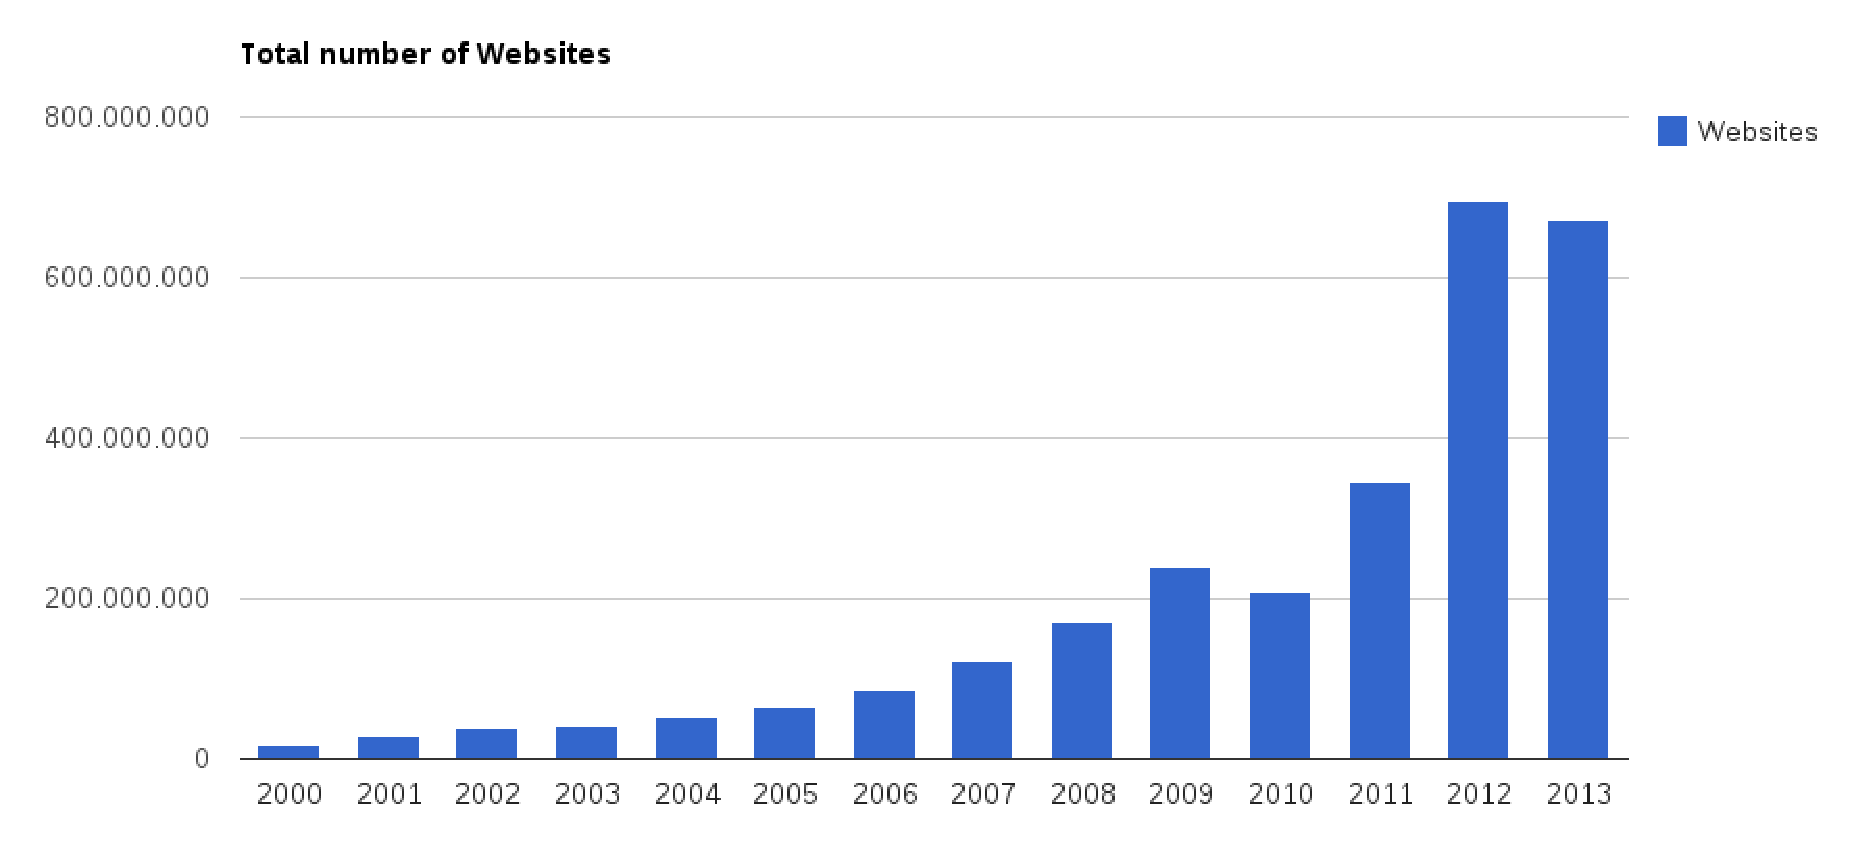
\includegraphics[width=0.9\textwidth]{numero_de_websites}
\caption{Número total de Websites por ano. Extraído de \cite{totalwebsite} }
\label{num-website}
\end{figure}

O grande problema desse avanço é que a maioria dos Websites criados ainda mantém sua característica inicial, ou seja, ainda são feitos para as pessoas interpretarem  e não as máquinas. De acordo com a Karin Breitman \cite{kbreitman}, essa Web atual pode ser definida como Web Sintática.

Segue um exemplo para que possamos entender melhor esse conceito: vamos supor que você esteja pensando em tirar umas férias. Você deseja visitar um lugar quente e tropical e reservou um orçamento de 3.000 reais para a sua viagem. Você deseja ficar em um bom lugar, mas não quer que isso custe muito em seu orçamento. Você também quer fazer um bom negócio com as passagens de avião \cite{web3}. 

Com os recursos da  Web (sintática) que temos atualmente, nós teríamos que pesquisar bastante para encontrarmos a melhor opção. Teríamos que visitar vários sites de passagens aéreas e de hotéis e ainda comparar os preços entre eles. Seria um processo muito trabalhoso.

Em \cite{kbreitman}, são enumerados os maiores problemas que temos com os atuais mecanismos de busca na Internet(nota rodape), através de ferramentas do tipo Google, Yahoo e Bing, por exemplo, como se segue:

\begin{itemize}
\item Grande numero de páginas encontradas, porém com pouca precisão – Por exemplo, ao realizar uma busca por TCP/IP no Google, temos aproximadamente 14.900.000 resultados. Mesmo encontrando páginas relevantes, esse resultado seria de pouca utilidade caso a maioria das páginas fossem de pouca relevância.
\item Resultados são muitos sensíveis ao vocabulário – em determinados casos, até a ordem em que as palavras são digitadas tem impacto nos resultados. Muitas vezes os documentos relevantes acabam usando terminologias diferente das nossas.
\item Resultados são páginas individuais – em muitos casos temos um grande número de páginas no resultado que pertencem a um mesmo site. Seria mais interessante ter algum tipo de organização geográfica dos resultados. Ao final, temos de extrair manualmente as porções desses documentos de interesse.
\end{itemize}

\graphicspath{{figuras/}}
\begin{figure}[H]
\centering
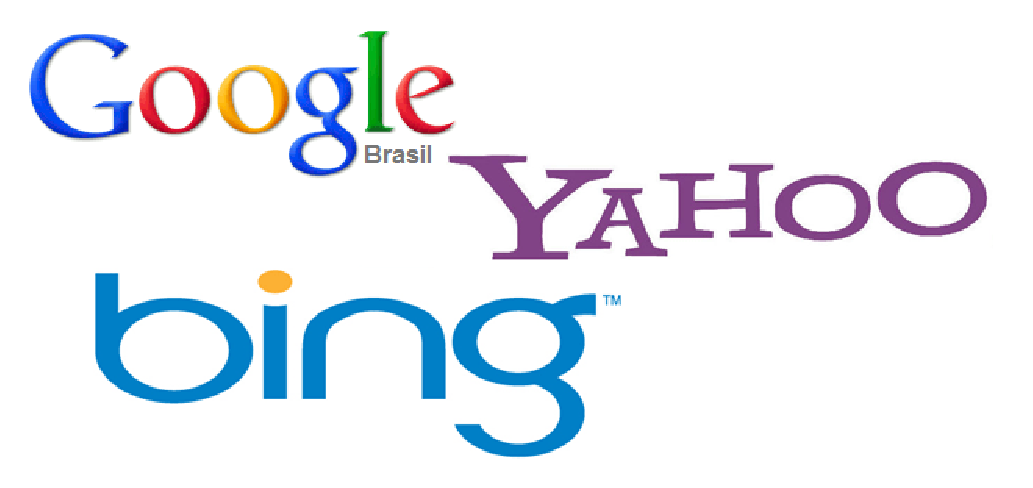
\includegraphics[width=0.7\textwidth]{Buscadores}
\caption{Buscadores web – principais meios de localização de informação. Extraído de \cite{intwebsem} }
\label{buscadores}
\end{figure}
O que podemos concluir dessas situações citadas acima, é que a Internet se tornou um meio para se compartilhar documentos entre pessoas, ao invés de ser um meio em que a troca de dados e informações pudessem ser processadas automaticamente.

No meio desse caos, Tim Berners-Lee, considerado por muitos o criador da Internet, apostou no aparecimento de uma Web mais organizada, mais conectada. Ele a chamou de Web Semântica.

De acordo com Bernes-Lee, Hendler e Lassila: “A Web Semântica é uma extensão da Web atual, na qual é dada à informação um significado bem definido, permitindo que computadores e pessoas trabalhem em cooperação”.

A ideia central é encontrar uma maneira de categorizar o conteúdo da Web de forma padronizada, facilitando seu acesso \cite{kbreitman}. A Web Semântica não se trata de uma nova rede de informações, mas sim de um projeto para aplicar conceitos inteligentes na internet atual. Nela cada informação vem com um significado bem definido e não se encontra mais solta no mar de conteúdo, permitindo uma melhor interação com o usuário.\cite{websemtecmundo}.


\section{Arquitetura da Web Semântica}

Não sabemos ainda como a web semântica será efetivamente construída, mas já existe uma arquitetura definida pela W3C (World Wide Web Consortium). Segue abaixo sua representação:

\graphicspath{{figuras/}}
\begin{figure}[H]
\centering
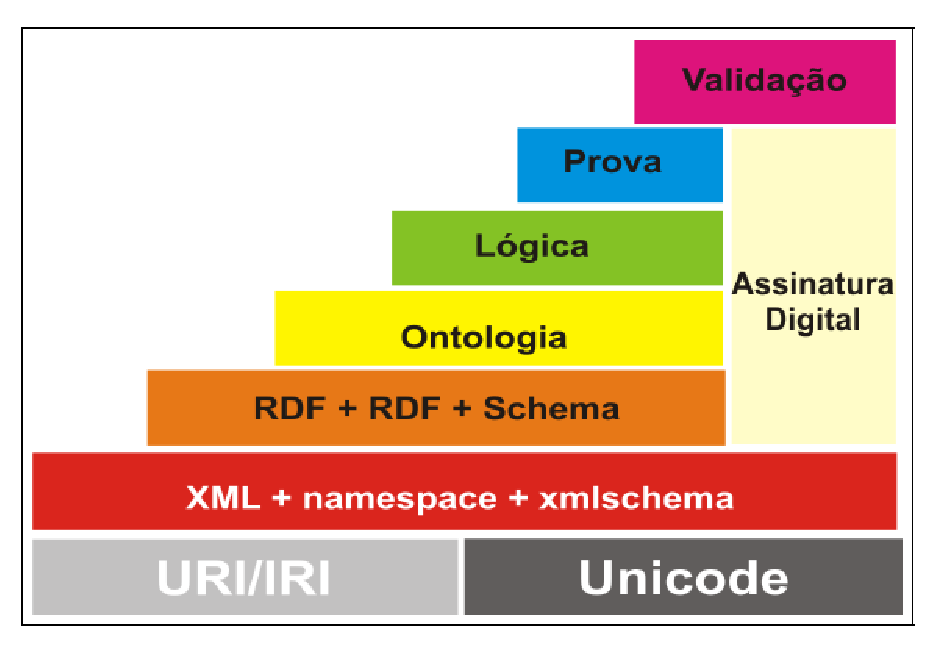
\includegraphics[width=0.8\textwidth]{arquitetura_web_semantica}
\caption[Arquitetura da Web Semântica]{Arquitetura da Web Semântica. Extraído de \cite{fig-arqweb}}
\label{arq_web_sem}
\end{figure}

Como podemos perceber, a arquitetura da web semântica é formada por 7 camadas, cada uma com uma ferramenta e tecnologia diferente (ALVES, 2003). Tim Berners-Lee, definiu uma estrutura em camadas que reflete os passos que devem ser dados para que o projeto da Web Semântica seja realizado de uma forma incremental \cite{ferneda}. As próximas seções falaram um pouco sobre essas sete camadas.

\subsection{URI/IRI e UNICODE}

Vamos realizar uma abordagem Top-Down(nota rodape), ou seja, vamos começar a análise pela camada mais inferior. Esta camada é composta pela URI (Uniform Resource Identifier) e UNICODE que são padrões para a descrição e estabelecimento de identificadores universais do recurso e códigos internacionais de dados \cite{santarem}. Esses dois elementos são responsáveis pela designação de uma identificação mínima dos recursos na rede \cite{vesu}.

Segundo \cite{elementoswebsem}, o URI é um padrão para identificar um recurso físico ou abstrato de maneira única e global. Ele estabelece uma forma padrão para a identificação de recursos. Através da utilização de URI faz-se a referência para recursos representados na Web Semântica. No contexto da Internet, o conceito de URI já é bem utilizado. Na Web é utilizado um tipo de URI chamado URL. Através da URL é possível endereçar documentos utilizando protocolos específicos da Internet como http e ftp \cite{rosa}.

Já o UNICODE, de acordo com \cite{rosa}, é uma linguagem que define uma forma padrão para a representação de caracteres. Unicode proporciona uma forma única para a representação de um caractere não importando a plataforma, o programa nem a linguagem que está sendo utilizada. A utilização de Unicode na Web Semântica proporciona a capacidade de troca de símbolos de maneira universal, requisito fundamental para o sucesso desta nova proposta de representação de informação na Internet. 

\subsection{XML, NAMESPACE e XML Schema}

Essa camada 2, também chamada de camada sintática, é responsável pelo estabelecimento correto da sintaxe de descrição dos dados.

O XML(nota rodape) é uma linguagem de marcação que, diferentemente do HTML, permite a criação e o uso de tags personalizadas, fornecendo assim uma maneira simples de organizar e estruturar os dados existentes em uma determinada aplicação \cite{XML2009}. Atualmente, o XML é a linguagem padrão recomendada pelo W3C(nota rodape) para troca de dados via Web.

Hoje, a Web Semântica exige uma descrição formal da semântica dos dados, de tal forma a evitar ambiguidades e permitir a interpretação de informações por parte das aplicações. Neste contexto, XML provê uma sintaxe bem definida, sendo atualmente utilizado na maioria das aplicações existentes na Web \cite{filholoscio}.

\graphicspath{{figuras/}}
\begin{figure}[H]
\centering
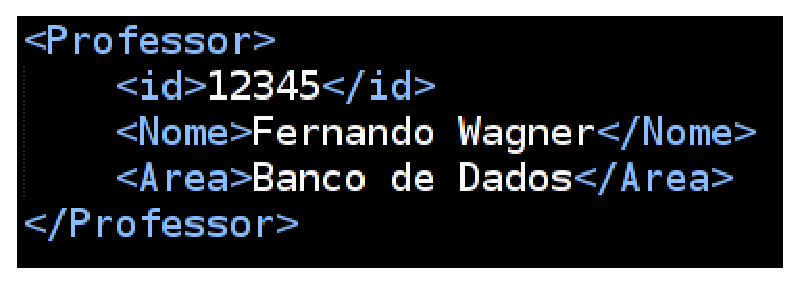
\includegraphics[width=0.6\textwidth]{xml1}
\caption{Trecho de código XML destacando dados de um professor.}
\label{xml1}
\end{figure}

\graphicspath{{figuras/}}
\begin{figure}[H]
\centering
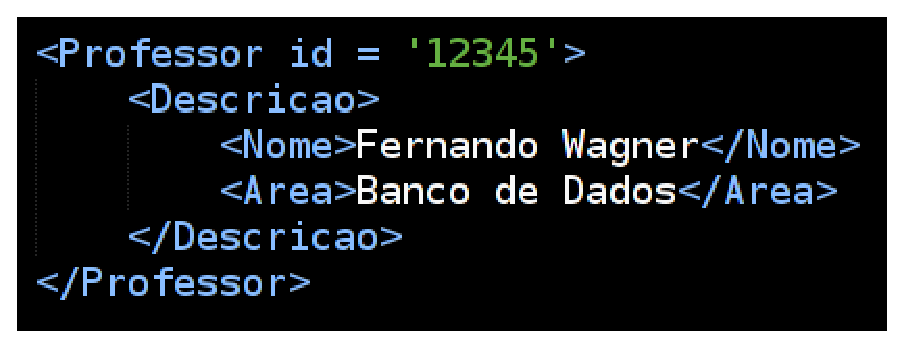
\includegraphics[width=0.6\textwidth]{xml2}
\caption{Documento XML alternativo ao da figura \ref{xml1}.}
\label{xml2}
\end{figure}

Um fato importante a ser levado em consideração no XML, é que um mesmo conjunto de dados podem ser representados de várias formas. Se observarmos figura \ref{xml2}, por exemplo, podemos perceber que ela é uma versão alternativa a figura \ref{xml1}. Essa característica pode causar algumas discordâncias entre aplicações. 

Para contornar esses problemas, foram criadas linguagens que definem esquemas para XML. São uma espécie de contrato, onde todas as partes envolvidas por um contexto de aplicação devem escrever seus documentos XML seguindo o padrão de estruturação especificado no esquema XML correspondente. Dentre as linguagens para definição de esquemas XML, destacam-se DTD e XML Schema \cite{filholoscio}.

De acordo com \cite{rosa}, XML Schema é uma ferramenta que permite a definição e a descrição de estruturas e de conteúdos de documentos XML. Através dessa linguagem, define-se o formato válido de um documento XML, incluindo quais elementos e atributos são permitidos ou não, quais são as suas localizações, o número de ocorrências de cada elemento e outras características. Ou seja, proporciona mecanismos para a definição de gramáticas para correção de documentos XML.

O último elemento dessa camada, são os chamados namespaces. Eles são classificados como um método para qualificar nomes de elementos e atributos usados em documentos XML, através da associação de referências URI. Através desse mecanismo de espaço de nomes, é possível a combinação de documentos com a utilização de vocabulário compartilhado. Através do mecanismo de espaço de nomes definido em XML, é possível compartilhar e reutilizar a definição de outros esquemas XML sem que haja problemas de colisão de nomes \cite{rosa} .

\subsection{RDF e RDF Schema}

Essa camada também pode ser chamada de camada de dados. Ela está diretamente relacionada com a representação, o processamento e a codificação dos metadados \cite{vesu}. Para isso estão presentes nessa camada a arquitetura de metadados RDF e o RDF Schema, que são ferramentas responsáveis por expressar significados e promover a interoperabilidade entre metadados e padrões ou formatos de metadados \cite{santarem}.